\chapter{Implementation}
\label{cha:Implementation}

\section{Generalising the Codebase}
\label{sec:Generalising the Codebase}
The first step in development was to modify the AIM4 codebase so that it could be more easily adapted to work with other simulations. This ended up being a more difficult task than expected and much of the code has been refactored out into general and AIM specific classes, in order to allow it to be extended effectively. There are still some artefacts left over in the generalised code from AIM, however the vast majority has been removed. 

Generalising the codebase was done in conjunction with Rebecca Milligan, who is also working on AV simulations in her car park management project.

\subsection{aim4.driver}
\label{subsec:aim4.driver}
Figure \ref{fig:driverBefore} is a class diagram indicating the structure of Driver and it's subclasses before changes were made. Figure \ref{fig:driverAfter} shows the structure in the generalised codebase.

\begin{figure}[htb]
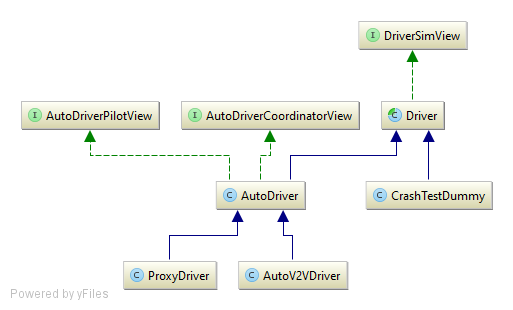
\includegraphics[width=\textwidth]{class_diagrams/driverBefore.png}
\caption{Original class structure for aim4.driver.}
\label{fig:driverBefore}
\end{figure}

\begin{figure}[htb]
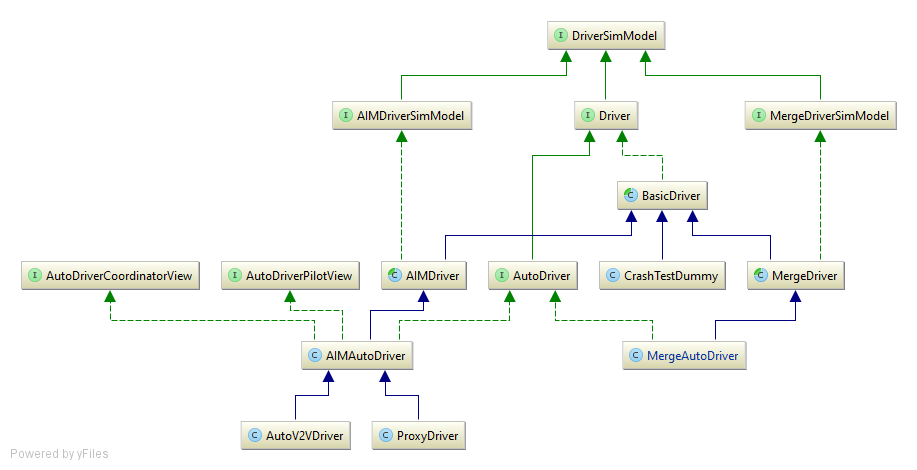
\includegraphics[width=\textwidth]{class_diagrams/driverAfter.png}
\caption{New class structure for aim4.driver, after changes were made generalising the codebase.}
\label{fig:driverAfter}
\end{figure}

The first major change was renaming \emph{DriverSimView}, \emph{AutoDriverPilotView}, and \emph{AutoDriverCoordinatorView} to end in \emph{Model} instead of \emph{View}. These interfaces are used to limit the methods that other classes can access in Driver and AutoDriver, thus changing their 'view' of that class. We didn't want to continue using \emph{View} as it could cause confusion with the GUI elements of the simulator. \revisit{We chose to refer to these interfaces as \emph{Models}, because the accessors are effectively given a model of Driver and AutoDriver (beyond which they care very little) that they can use to access the methods they want.}

The next change was separating out all of the AIM specific code into its own classes and interfaces. You can see how this was done in Figure \ref{fig:driverAfter} with AIMDriverSimModel and AIMDriver. By extracting AIM specific behaviour, we created general classes that could be extended, reducing code duplication. The merge specific code found in MergeDriverSimModel, MergeDriver and MergeAutoDriver is structured in a very similar manner to its AIM counterpart, taking advantage of the generalised code. However, as a consequence of breaking out the code like this, a number of additional changes had to be made. 

\revisit{Driver was broken out into an interface and a new class BasicDriver. Driver is simply used as an interface for accessing Drivers in non-simulation contexts (such as Vehicle). BasicDriver contains the generalised functionality all Drivers are required to have, with AIM specific activities moved to AIMDriver. Extending from Driver is the AutoDriver interface, which adds no new methods but is instead used to categorise autonomous drivers. AIMAutoDriver contains almost exactly the same code as the original AutoDriver class.}

\subsection{aim4.gui}
\label{subsec:aim4.gui}
In the original simulator, shown in Figure \ref{fig:originalAIMSetupLabeled} Viewer.mainPanel displays the simulator setup and canvas using a CardLayout. In the new GUI, shown in Figure \ref{fig:newAIMSetupLabeled} we replaced mainPanel with tabbedPane, a JTabbedPane object that allows users to switch between different simulators. On each tab we added a SimViewer object, shown in Figure \ref{fig:simViewer}, which behaves in the same way that mainPanel did in the original code. Each SimViewer has two panels, a SimSetupPanel and a SimScreen, which it can switch between using CardLayout. Functionality from SimSetupPanel was extracted out into separate AIM specific and general classes. It is used to create and modify SimSetup objects. SimScreen is a new interface which Canvas inherits from. It is used to allow SimViewers to display objects other than Canvas instances, such as MergeStatScreen, when the simulation is run. You can see how SimSetupPanel and SimScreen are structured in Figures \ref{fig:simSetupPanel} and \ref{fig:simScreen}.

\begin{figure}[htb]
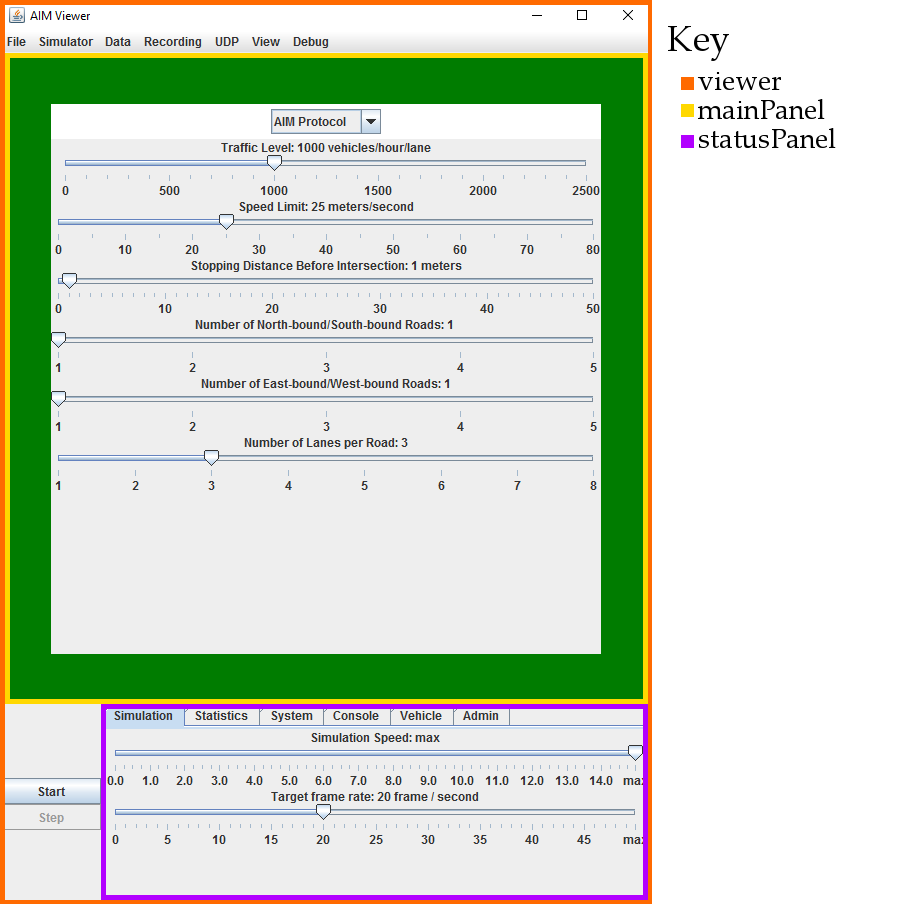
\includegraphics[width=\textwidth]{screenshots/originalAIMSetupLabeled.png}
\caption{Panel layout in the original Viewer}
\label{fig:originalAIMSetupLabeled}
\end{figure}

\begin{figure}[htb]
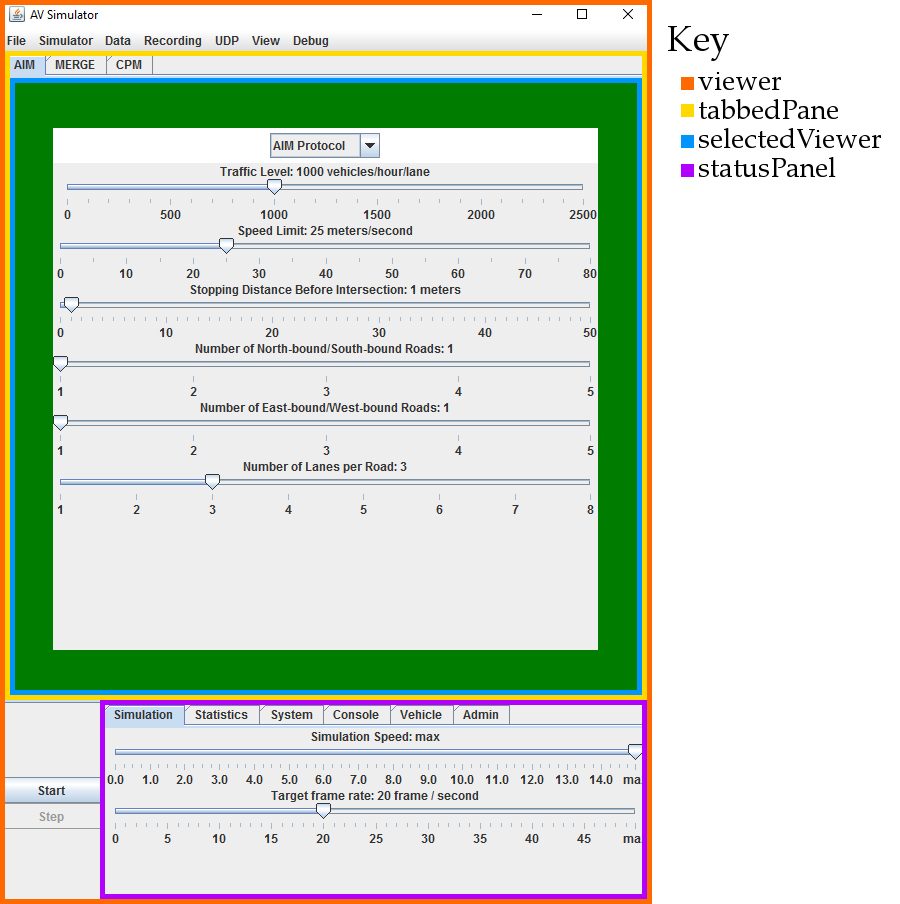
\includegraphics[width=\textwidth]{screenshots/newAIMSetupLabeled.png}
\caption{Panel layout in the new Viewer}
\label{fig:newAIMSetupLabeled}
\end{figure}

\begin{figure}[htb]
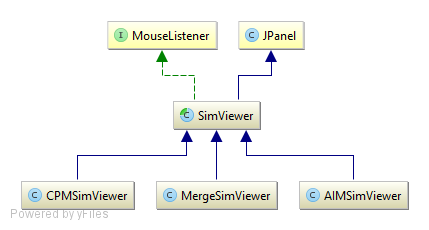
\includegraphics[width=\textwidth]{class_diagrams/simViewer.png}
\caption{The class diagram for SimViewer}
\label{fig:simViewer}
\end{figure}

\begin{figure}[htb]
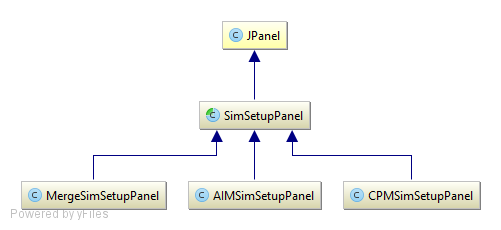
\includegraphics[width=\textwidth]{class_diagrams/simSetupPanel.png}
\caption{The class diagram for SimSetupPanel}
\label{fig:simSetupPanel}
\end{figure}

\begin{figure}[htb]
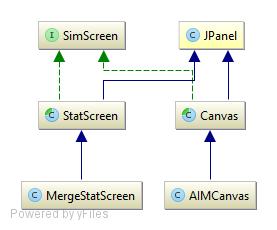
\includegraphics[width=\textwidth]{class_diagrams/simScreen.png}
\caption{The class diagram for SimScreen}
\label{fig:simScreen}
\end{figure}

We also made a small adjustment to the behaviour of the reset option in the menu. The simulator must be paused in order for the reset button not be greyed out.

\subsection{aim4.map}
\label{subsec:aim4.map}


\begin{figure}[htb]
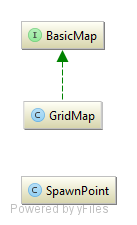
\includegraphics[width=\textwidth]{class_diagrams/mapBefore.png}
\caption{The original class structure for BasicMap and SpawnPoint.}
\label{fig:mapBefore}
\end{figure}

\begin{figure}[htb]
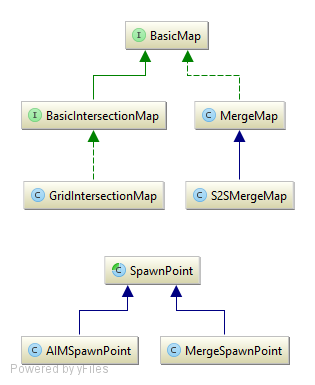
\includegraphics[width=\textwidth]{class_diagrams/mapAfter.png}
\caption{The new class structure for BasicMap and SpawnPoint.}
\label{fig:mapAfter}
\end{figure}